\documentclass[tikz, border=10pt]{standalone}
\usepackage{tikz}
\usetikzlibrary{calc}

\begin{document}
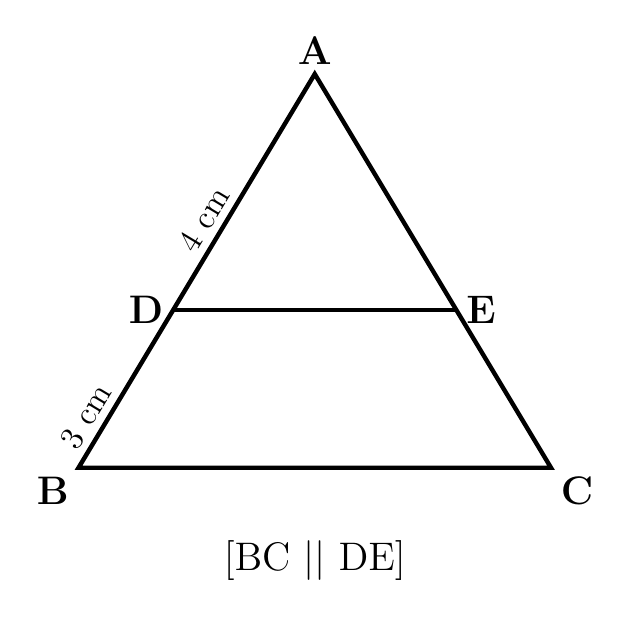
\begin{tikzpicture}

% Define vertices of main triangle
\coordinate (A) at (3, 5);
\coordinate (B) at (0, 0);
\coordinate (C) at (6, 0);

% Define D and E on sides AB and AC (parallel to BC)
\coordinate (D) at ($(B)!0.4!(A)$);
\coordinate (E) at ($(C)!0.4!(A)$);

% Draw the main triangle ABC
\draw[ultra thick] (A) -- (B) -- (C) -- cycle;

% Draw the parallel line DE
\draw[ultra thick] (D) -- (E);

% Labels for vertices
\node[above] at (A) {\textbf{\Large A}};
\node[below left] at (B) {\textbf{\Large B}};
\node[below right] at (C) {\textbf{\Large C}};
\node[left] at (D) {\textbf{\Large D}};
\node[right] at (E) {\textbf{\Large E}};

% Dimension label: AD = 4 cm (along line AD)
\coordinate (midAD) at ($(A)!0.5!(D)$);
\node[above left, font=\large, rotate=59] at (midAD) {4 cm};

% Dimension label: DB = 3 cm (along line DB)
\coordinate (midDB) at ($(D)!0.5!(B)$);
\node[above left, font=\large, rotate=59] at (midDB) {3 cm};

% Label showing BC || DE
\node[below, font=\Large] at (3, -0.8) {[BC $\mid\mid$ DE]};

\end{tikzpicture}
\end{document}